\chapter{Ergebnisse und Diskussion}

Im Fokus dieses Kapitels stehen die Ergebnisse und Diskussionen im Kontext der Evaluierung von Dichteeigenschaften. Schrumpfungsverhalten und mechanische Kennwerte des 316L-Edelstahls von \textit{PT+A} für den 3D-Druck mittels FDM. Im vorangegangenen Kapitel wird die Erstellung der Proben und die wissenschaftlichen Grundlagen erläutert.

\section{Dichte- und Schwindungsauswertungen der gedruckten Proben}
\label{Dichte- und Schwindung}
In diesem Unterkapitel werden die gedruckten Würfel- und Zugproben hinsichtlich der Dichte untersucht. Diese Messung wird zuerst im Grün-, sowie im Braun-, als auch im späteren Sinterteil durchgeführt, damit die Schwindungen und die Massenverluste bestimmt werden kann. Die Ergebnisse dieser Auswertung ist in \autoref{Grünteilmaße} bis \autoref{Sinterteilmaße} dargestellt. Die Durchschnittswerte sind in \autoref{tab:Rohdaten} dargestellt. Sie geben einen Überblick über die das Verhalten der Würfel in jedem der drei Zustände.
Aus diesen Werten lassen sich die Schwindungen der einzelnen Parameter nach jedem Prozess ableiten. Dargestellt sind diese Werte in \autoref{tab:Schrumpfung}. Dargestellt sind hier die relative Schrumpfungen/Zunahmen in Vergleich zum Grünteil.\\
Die Ergebnisse der Dichtemessung ist in \autoref{DichtewerteTestwürfel} visuell dargestellt. Im Durchschnitt beträgt die Dichte 6,87 \(\text{g/cm}^3\). Nachfolgend werden diese Werte mit dem Datenblatt und anderen Studien verglichen. Es wird ebenfalls erklärt, wie das Verhalten zustande kommt.

\begin{figure}[h] 
  \centering
  \includegraphics[width=0.8\linewidth]{bilder/img_Dichtewerte der Testwürfel.png}
        \caption[Dichtewerte der Testwürfel als Metallteil] {Dichtewerte der Testwürfel als Metallteil (Quelle: eigene Darstellung)}
  \label{DichtewerteTestwürfel}
\end{figure}
%\FloatBarrier


\begin{table}[h]
  \centering
  \caption{Datentabelle der Würfelproben}
  \captionsetup{font=small} % Schriftgröße auf small setzen
  \footnotesize
  \begin{tabular}{ccccccc}
    \toprule
    \textbf{Teil} & \multicolumn{1}{c}{\textbf{Z [mm]}} & \multicolumn{1}{c}{\textbf{X [mm]}} & \multicolumn{1}{c}{\textbf{Y [mm]}} & \multicolumn{1}{c}{\textbf{Volumen [mm\(^3\)]}} & \multicolumn{1}{c}{\textbf{Masse [g]}} & \multicolumn{1}{c}{\textbf{Dichte [g/cm\(^3\)]}} \\
    \textbf{Grünteil} & 9,99 & 10,17 & 10,19 & 1035,89 & 4,75 & 4,59 \\
    \textbf{Braunteil} & 10,00 & 9,88 & 9,90 & 977,29 & 4,52 & 4,62 \\
    \textbf{Sinterteil} & 8,62 & 8,60 & 8,58 & 636,20 & 4,37 & 6,87 \\
    \bottomrule
  \end{tabular}%
  \label{tab:Rohdaten}%
\end{table}%
\FloatBarrier

\begin{table}[h]
    \centering
    \caption{Schrumpfung der Würfelproben im Braun- und Sinterteil}
      \begin{tabular}{ccccccc}
      \toprule
      \textbf{Teil} & \multicolumn{1}{c}{\textbf{Z [\%]}} & \multicolumn{1}{c}{\textbf{X [\%]}} & \multicolumn{1}{c}{\textbf{Y [\%]}} & \multicolumn{1}{c}{\textbf{Volumen [\%]}} & \multicolumn{1}{c}{\textbf{Masse [\%]}} & \multicolumn{1}{c}{\textbf{Dichte [\%]}} \\
        \textbf{Entbindern} & 0 & -2,9 & -2,9 & -5,8 & -4,8 & 0,8 \\
        \textbf{Sintern} & -13,7 & -15,4 & -15,8 & -38,6 & -8 & 50 \\
      \bottomrule
      \end{tabular}%
    \label{tab:Schrumpfung}%
  \end{table}%
  \FloatBarrier

Wie in \Autocite{Industrie4} und in \autoref{fig:Verlust} dargestellt, ist die Volumenschrumpfung nach dem Entbindeprozess deutlich geringer, als im Sinterprozess. Grund hierfür ist der Binder, der durch das Lösemittel gelöst wird. Dadurch entstehen verhältnismäßig kleine Volumenschwindungen. Die Metallpartikel liegen wenig verändert in dem selben Gefüge, das erklärt ein Volumeverlust von 5,8 \%. Nach dem Sintern rücken die Metallpartikel deutlich dichter zueinander, was zu einer Volumenschrumpfung von 38,6 \% führt. Der Verlust der Masse beträgt im Entbindeprozess 4,8 \% und im Sinterprozess 8 \%. Bei der Veränderung der Masse sieht es anders aus. Die Erklärung liegt in der Vorgehensweise des Entbindern. Das Lösemittel diffundiert in das Grünteil hinein und löst das Bindemittel. Dabei wird ein großer Teil abgetragen, dieser liegt aber hauptsächlich in der Randzone der Würfel (siehe \autoref{fig:Verlust}). In dieser Arbeit beläuft sich der Abtrag des Bindemittels aus dem Entbindeprozess knapp über die Hälfte des gesamten Massenverlustes.Nach dem Entbindern bleibt ein Gerüst aus Bindemittel, welches die Geometrie für das Sintern zusammenhält. Dies nennt man auch Rückgrat\textit{engl. Backbone} \Autocite{Industrie4}.
Im Sinterprozess wird dieser Rest an Binder entfernt. Dies führt dann zu einem Gewichtsverlust von 8 \%. \textbf{VERGLEICH?}\\
Die Dichte nimmt über beide Prozessschritte zu. Somit ist sie der einzige Parameter, der nicht abschrumpft, sondern zunimmt. Diese Entwicklung lässt sich darauf zurückführen, dass das Volumen deutlich stärker schrumpft als die Masse. Die Dichte, die durch die Division des Volumens durch die Masse berechnet wird, erfährt daher eine Steigerung.

\begin{figure}[h] 
  \centering
  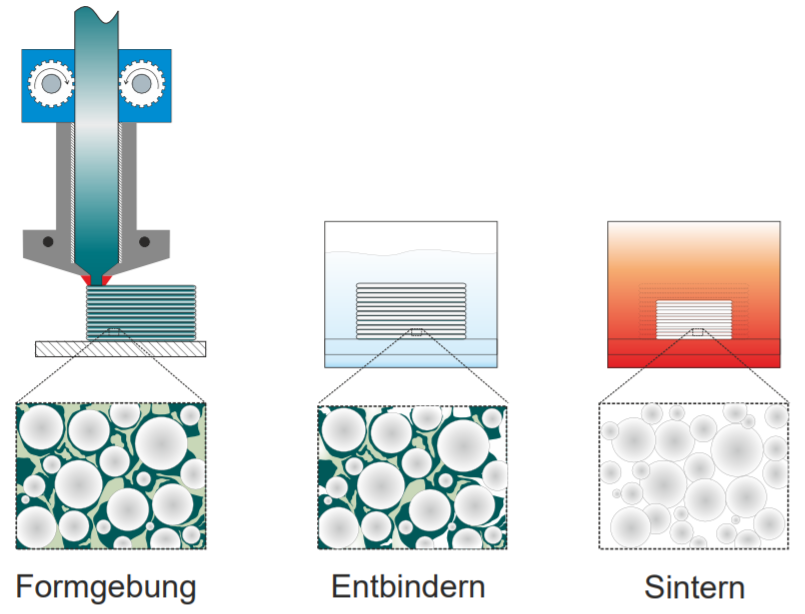
\includegraphics[width=0.8\linewidth]{bilder/Kukla_Bild1.png}
        \caption[Darstellung Formgebung, Entbindern und Sintern] {Darstellung Formgebung, Entbindern und Sintern \autocite{Industrie4}}
  \label{fig:Verlust}
\end{figure}

Von den liegenden Zugproben wurden auch Masse und Gewicht gemessen. Daher lassen sich auch hier das Schrumpfungsverhalten darstellen. Diese Werte sind in \autoref{Schrumpfung Zugproben} angegeben. Dabei decken sich die Schrumpfung des Volumens mit denen der Würfel. Lediglich die Schrumpfung der Masse ist mit 12 \% genau 4 Prozentpunkte mehr als bei den Würfeln. Dies ist ein Zeichen für eine effektivere Entbinderphase. \textbf{Dichte der Zugproben ermitteln und einf.}


\begin{table}[h]
    \centering
    \caption{Schrumpfung der liegenden Zugproben im Sinterteil}
      \begin{tabular}{ccccccc}
      \toprule
      \textbf{Prozess} & \multicolumn{1}{c}{\textbf{Volumen [\%]}} & \multicolumn{1}{c}{\textbf{Masse [\%]}} & \multicolumn{1}{c}{\textbf{Dichte [\%]}} \\
        \textbf{Sinterteil} & -38,4 & -12 & +42,9 \\
      \bottomrule
      \end{tabular}%
    \label{Schrumpfung Zugproben}%
  \end{table}%
  \FloatBarrier

\section{Ergebnisse der Zugversuche}

In diesem Abschnitt werden die mechanischen Kennwerte des 316L-Edelstahls mittels eines Zugversuchs ermittelt. Dazu wird mithilfe des, in \autoref{Drucker} vorgestellten, FDM-Drucker Zugproben hergestellt. Diese Zugproben sind nach DIN 50125-E3x8x30 hergestellt.
Ziel dieser Arbeit ist ein Vergleich zwischen zwei verschiedene Ausrichtungen dieser Proben.
\begin{figure}[h] 
  \centering
  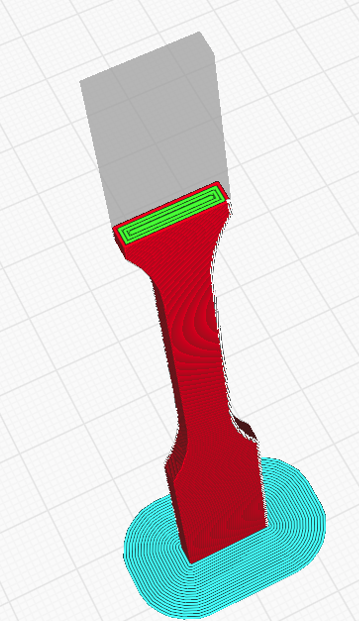
\includegraphics[width=0.4\linewidth]{bilder/Screenshot 2023-11-01 171423.png}
        \caption[Stehende Zugprobe im Cura-Slicer] {Stehende Zugprobe im Cura-Slicer (Quelle: \autocite{Prusa})}
  \label{stehende Zugprobe}
\end{figure}
\FloatBarrier

\textbf{WARUM VERGLEICH STEHENDE LIEGENDE ZUGPROBEN}
Die Orientierung der Werkstücke in der Slicing-Software spielt eine große Rolle. Um diese Unterschiede sichtbar zu machen, wird in dieser Arbeit der Vergleich zwischen \glqq liegenden\grqq und \glqq stehenden\grqq Zugproben angestellt. Die \glqq liegenden\grqq Zugproben liegen flach auf dem Druckbett, was zu großen Druckflächen pro Druckschicht führt (siehe \autoref{fig:liegendeZugproben}). Verglichen mit dieser Fertigungsmethode werden \glqq stehende\grqq Zugproben. In diesem Fall werden die Zugproben auf ihrer kleinsten Fläche aufgestellt (siehe \autoref{fig:stehendeZugproben}). Mit dieser Methode werden kleinere Flächeninhalte als bei den \glqq liegenden\grqq Zugproben erreicht.

Beim Zugversuch werden jeweils die dickeren Enden der Zugprobe in eine Vorrichtung eingespannt. Die Zugmaschine bringt eine Kraft an beide Enden auf, die dann eine Längung verursacht, die dann bis zum Bruch führt.\\
Von Interesse ist in dieser Arbeit der Unterschied zwischen eine Kraft die längs der Druckschicht angebracht ist (siehe \autoref{fig:Kraftlängs}), zu einer Kraft die quer an die Druckschicht angebracht wird (siehe \autoref{fig:KraftQuer}). \textbf{Unzufriedener Satzbau}
Dieser Vergleich bringt Aufschluss über Optimierungsmöglichkeiten, die über Orientierung der Werkstücke erreicht werden kann. Ausserdem werden die erreichten Werte in \autoref{sec:Vergleich} mit dem Datenblatt und anderen Quellen verglichen.

Da die Querschnittsfläche einer stehenden Zugprobe deutlich kleiner ist, als bei den liegenden Zugproben, führt dies zu dem Phänomen, dass die zuvor gedruckte Schicht nicht direkt abkühlen kann, ehe dann die nächste Schicht gedruckt wird. Es ist gelungen stehende Zugproben zu drucken, indem die Druckgeschwindigkeit deutlich verringert und die Lüfterdrehzahl auf 60 \% reduziert ist. Jedoch sind die Proben beim Versand zu \textit{L.B. Bohle} in dem Päckchen zerstört. Daher wird sich im Rahmen dieser Arbeit auf den Vergleich zwischen den liegenden Zugproben hinsichtlich der mechanischen Kennwerte bezogen.
Im Slicer sind dann in x- und y-Richtung um 17 \% vergrößert und in z-Richtung sind sie 20 \% größer gedruckt. Damit ist sichergestellt, dass die Zugproben im gesinterten Zustand die DIN-Norm einhalten. Die fertig gesinterten Zugproben werden dann in eine Zugprüfmaschine an beide Seiten eingespannt und bis zur Zerstörung gezogen. Die benötigte Kraft, sowie die entstehende Längung bilden die Grundlage für das entstehende Spannungs-Dehnungs-Diagramm.
Das zugehörige Spannungs-Dehnungs-Diagramm ist in \autoref{ZugprobenS} dargestellt, anzumerken ist an dieser Stelle, dass nur \autoref{ZugprobenS} Zugproben enthält, die im Rahmen dieser Arbeit gedruckt sind. Die anderen drei Ergebnisse \autoref{ZugprobenGS}, \autoref{ZugprobenP} und \autoref{ZugprobenT} sind Zugproben, die in der Firma \textit{L.B. Bohle} gedruckt sind. Sie dienen nur als Vergleich.
 
\section{Vergleich der ermittelten Werte}
\label{sec:Vergleich}

\subsection{Vergleich der Dichte}

Die errechnete, durchschnittliche Dichte aus \autoref{Dichte- und Schwindung} beträgt 6,87 \(\text{g/cm}^3\). Verglichen mit dem technischen Datenblatt aus \autoref{Datenblatt1.4404} ist die Dichte dort mit 8 \(\text{g/cm}^3\) angegeben. Dies entspricht einer Abweichung von -14 \%. In \Autocite{Quarto.2021} wurde ebenfalls die Dichte an FDM-gedruckten Stahlteilen gemessen, hier lag sie im Durchschnitt bei knapp über 7,2 \(\text{g/cm}^3\). Dies entspricht einer Abweichung von -10 \%. Dieser Wert ist mit den Ergebnissen dieser Arbeit nur bedingt vergleichbar. In \autocite{Quarto.2021} wurde mit \textit{Ultrafuse} von \textit{BASF} gearbeitet. Das Material entspricht ebenfalls Edelstahl der Norm 1.4404. Die Abweichungen von Soll- und Istwerten werden mit \autoref{Abweichungen} errechnet.

\begin{equation}
  \text{Prozentuale Abweichung} = \left( \frac{\text{Soll-Dichte} - \text{Ist-Dichte}}{\text{Soll-Dichte}} \right) \times 100
  \label{Abweichungen}
\end{equation}
  


\subsection{Vergleich der Werte aus dem Zugversuch}

In \autoref{tab:ErgebnisseZugversuch} sind die relevantesten Ergebnisse aus den Zugversuchen aufgelistet. R$_{\textsubscript{p0.2}}$ stellt die Streckgrenze dar. R$_{\textsubscript{m}}$ steht für die Zugfestigkeit und A$_{\textsubscript{25 mm}}$ gibt die Bruchdehnung an. Verglichen werden hier die Werte für die Zugversuche der liegend gedruckten Proben. In der ersten Zeile sind die Proben, die im Rahmen dieser Arbeit gedruckt wurden aufgelistet \textit{(FH-Münster)}. In der zweiten Zeile sind die Proben der Firma \textit{L.B. Bohle} dargestellt. In der letzten Zeile \glqq Abweichungen\grqq sind die Abweichungen der ersten und zweiten Zeile von dem Datenblatt dargestellt.

\begin{table}[h]
  \centering
  \caption{Ergebnisse Zugversuch}
  \begin{tabular}{cccc}
  \toprule
  \textbf{Serie} & \textbf{R$_{\textsubscript{p0.2}}$ [MPa]} & \textbf{R$_{\textsubscript{m}}$ [MPa]} & \textbf{A$_{\textsubscript{25 mm}}$ [mm]} \\
  \midrule
  liegend (FH-MS) & 157 & 346 & 23,2 \\
  liegend (L.B. B.) & 178 & 400 & 25,4 \\
  Datenblatt 1.4404 \autocite{AGSTSteel:1.4404} & $\leq$ 200 & 500-700 & 40 \\
  \midrule
  Abweichungen (\%) 
    & -21,5 & -31,2 & -42,0 \\
    & -11,0 & -20,0 & -37,5 \\
  \bottomrule
  \end{tabular}
\label{tab:ErgebnisseZugversuch}
\end{table}

